%************************************************
\chapter{Simulation}\label{kap:simulation}
%************************************************
\section{IEEE 802.15.4 Modell}\label{kap:simulation_sec:beschreibung}
Beschreibung, Aufbau \\
Besonders wichtig : Modellierung des Funkkanals \\
Beschreibung des Fehlers in der Datensammlung für Kollisionen \\
Bewertung des Modells für die Verwendung in dieser Arbeit \\

\section{Erweiterungen des Modells}\label{kap:simulation_sec:erweiterung}
Austausch/Neuerstellung der Anwendungsschicht \\
Ergänzung um automatische, zufällige Platzierung der Container \\
Besonders wichtig: Anpassung der Transceivermodi -> Energiemodell \\
--> Einbindung realer Messwerte \\

\section{Simulationsergebnisse}\label{kap:simulation_sec:ergebnisse}
\begin{figure}[bth]
        \myfloatalign
        {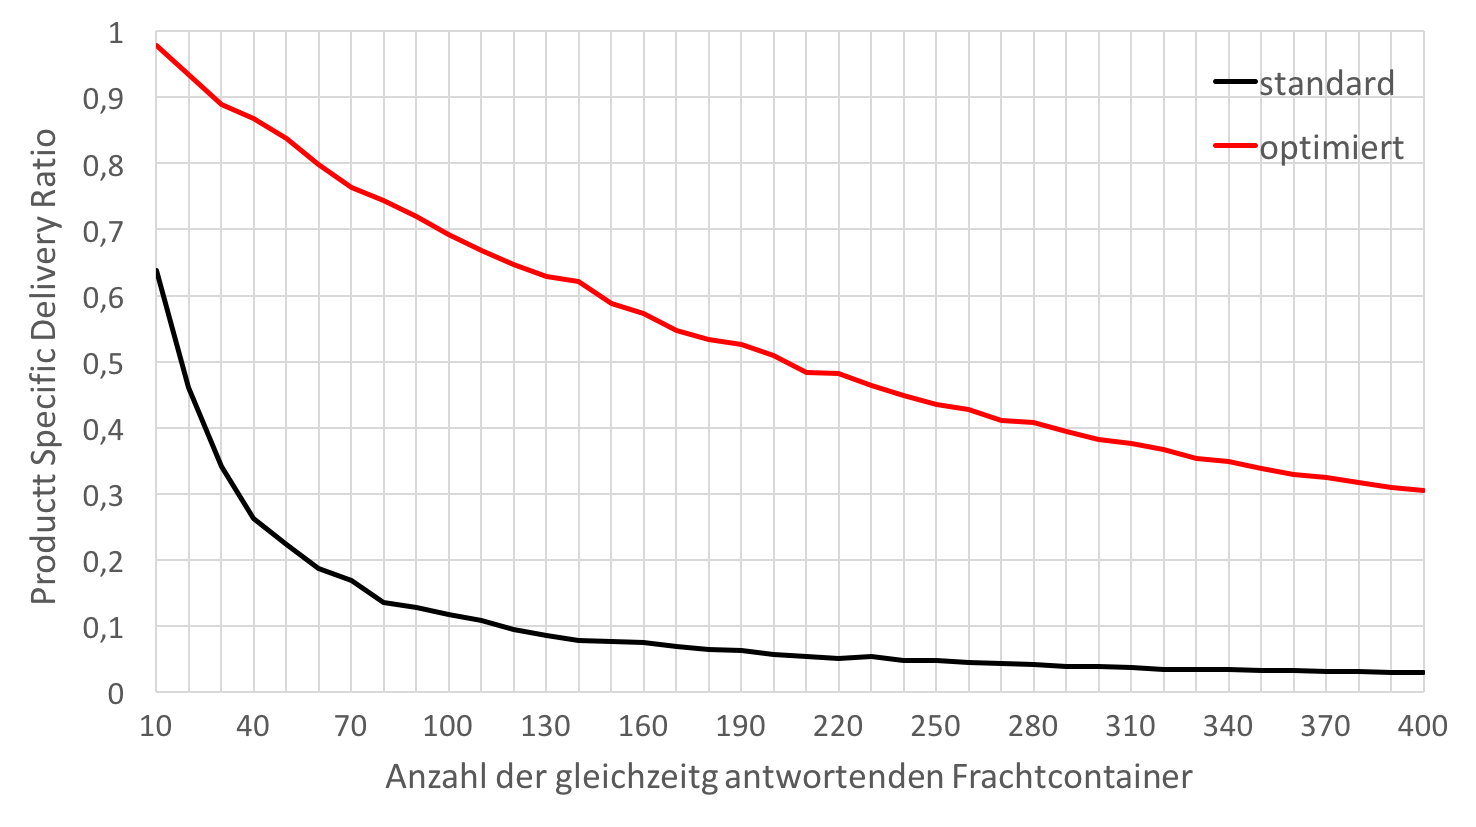
\includegraphics[width=1\linewidth]{gfx/Diag_Durchsatz_10_400}} 
        \caption[Durchsatz]{ToDo}\label{fig:diag_durchsatz_10_400}
\end{figure}

Beschreibung -> näherungsweise neg.exp. \\
Konvergenz interessant evtl. noch ein Durchlauf bis 1000 \\
Begründung des höheren Durchsatzes: Erleuterung der Auswahl von BE \\
evtl. Statistik mit einbeziehen \\

\begin{figure}[bth]
        \myfloatalign
        {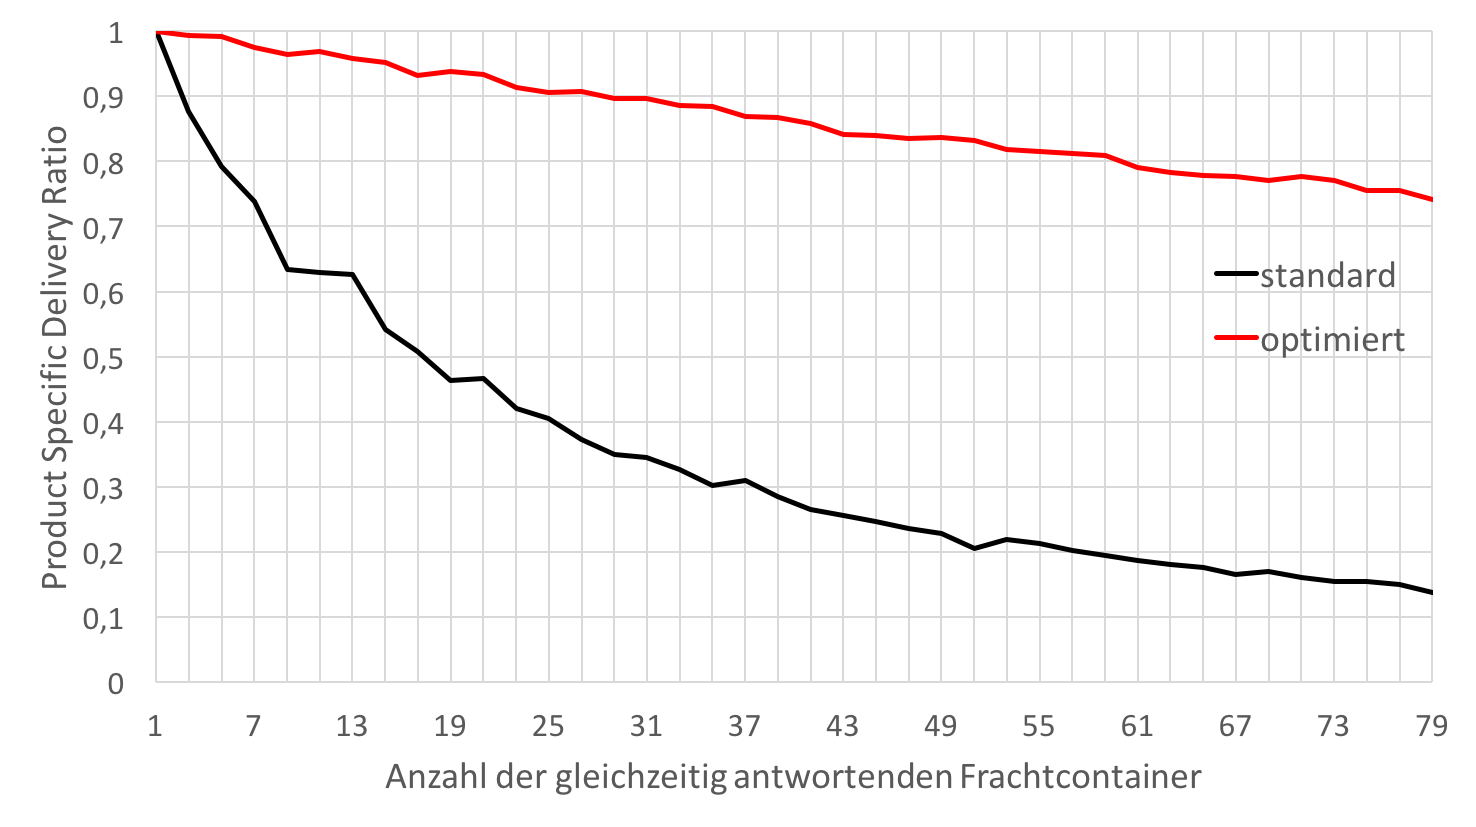
\includegraphics[width=1\linewidth]{gfx/Diag_Durchsatz_1_80}} 
        \caption[Durchsatz im Detail]{ToDo}\label{fig:diag_durchsatz_1_80}
\end{figure}

besonders effizient im Bereich bis ca. 80 Sendern \\
bei standard bereist bei wenigen Sendern massive Kollisionen

\begin{figure}[bth]
        \myfloatalign
        {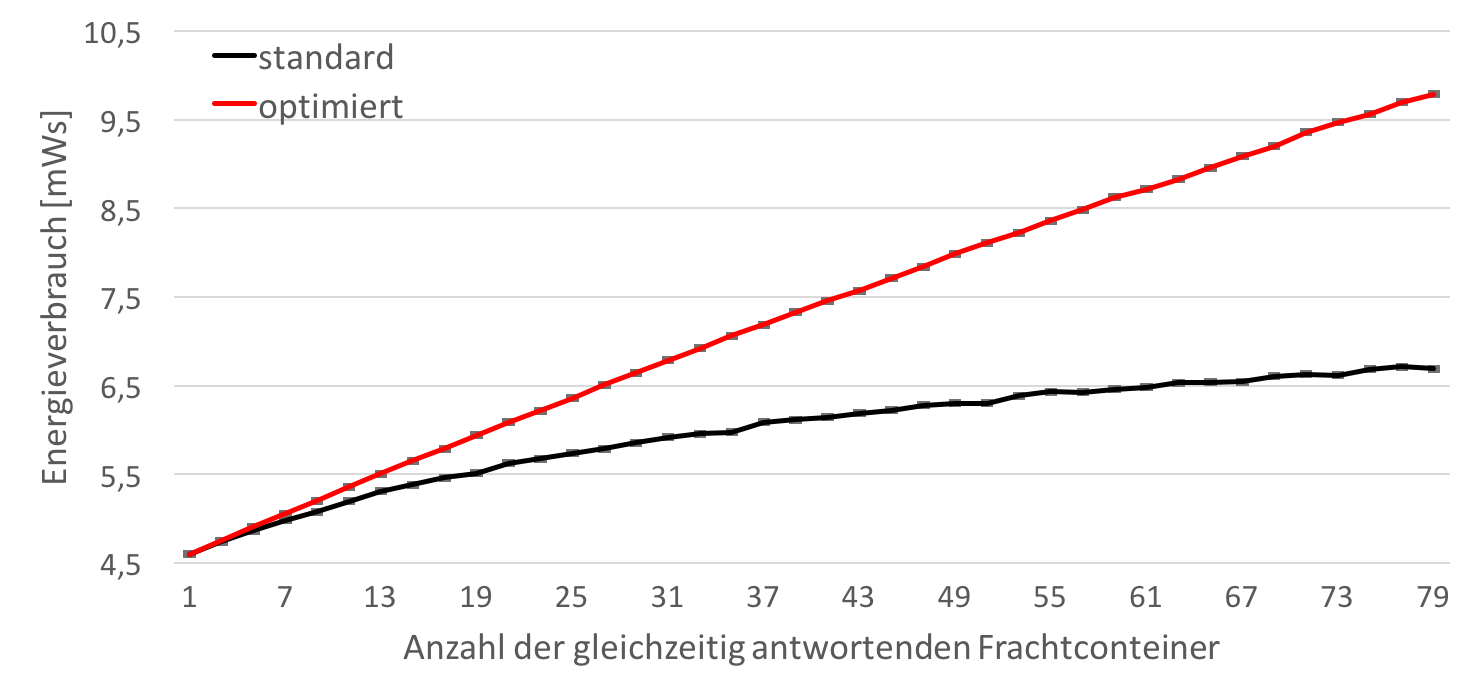
\includegraphics[width=1\linewidth]{gfx/Diag_Energie_1_80}} 
        \caption[Energieverbrauch]{ToDo}\label{fig:diag_Energie_1_80}
\end{figure}

Hinweis auf Energieverbrauch pro Sender während gesamter Laufzeit \\
Bezug von Energieverbruach auf erfolgreich zugestellte Nachrichten\\
--> dazu evtl. noch ein Diagramm \\
Energieverbrauch pro Sendeversuch \\

\begin{figure}[bth]
        \myfloatalign
        \subfloat[standard]
         {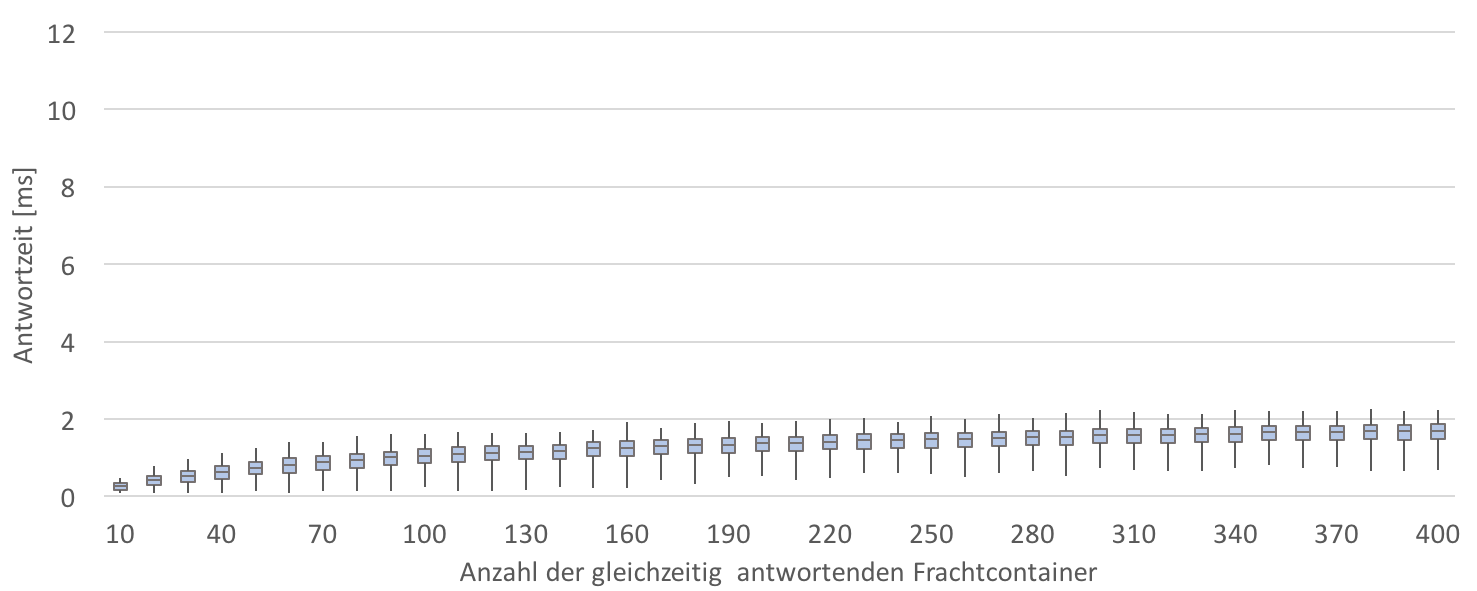
\includegraphics[width=1\linewidth]{gfx/Diag_Delay_std}} \\
        \subfloat[optimiert]
        {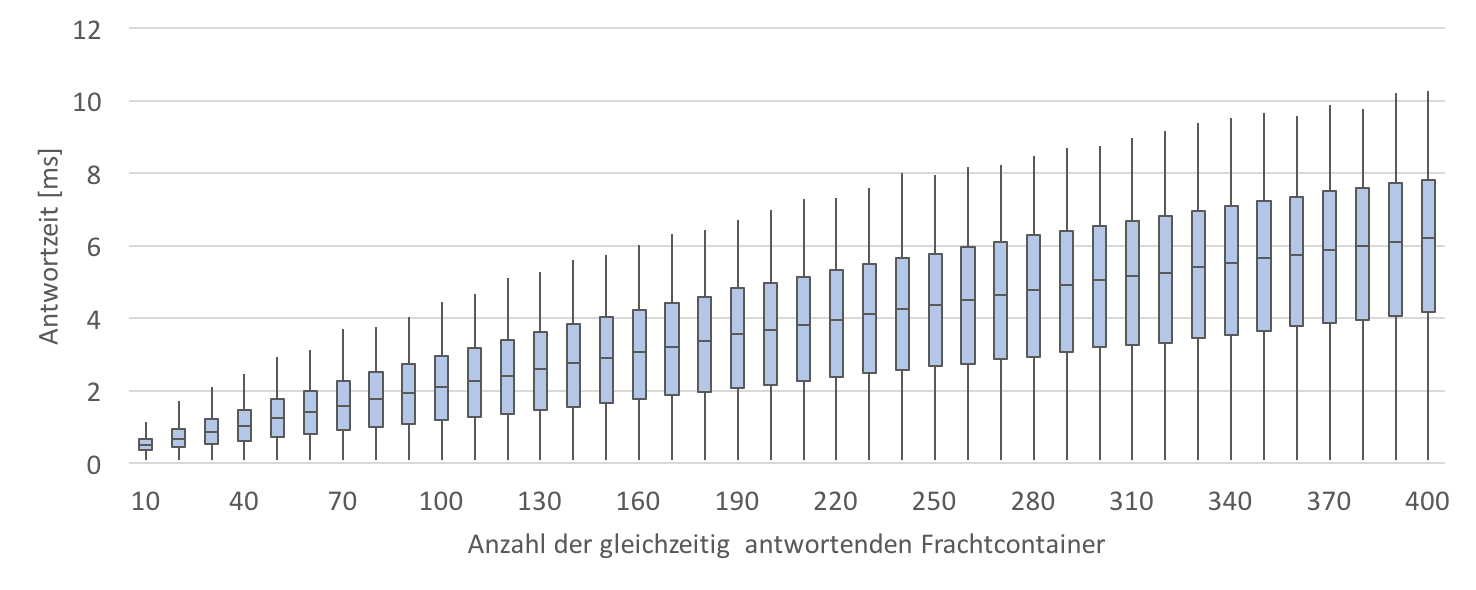
\includegraphics[width=1\linewidth]{gfx/Diag_Delay_opt}} 
        \caption[Verzögerung]{Boxplots der Antwortverzögerungen durch den \gls{csma} Algorithmus}\label{fig:diag_delay_1_400}
\end{figure}

Auswirkung der Algorithmus auf Antwortzeiten \\
Bezug und Bewertung dieses Effekts für das gegebene Szenario\\
Angabe von theoretischer oberer Schrake !? \\
Hinweis auf geringe Anzahl der Antworten insgesamt bei standard, wegen massiver Kollisionen
Hinweis zur Verteilung der einzelnen Antworten beim optimierten Verfahren\\
--> immer auch Anworten direkt nach Anfrage (Ausreißer nahe 0) --> effektive Kanalnutzung \\
dazu evtl noch Histogramm




%*****************************************
%*****************************************
%*****************************************
%*****************************************
%*****************************************




